\subsection*{Questão 08}

\textit{O que indica a frequência de um sinal?}\par

\textbf{Resposta: } 
A frequência de um sinal $f$ indica quantos ciclos um sinal periódico completa em um determinado intervalo de tempo, normalmente um segundo, conforme o padrão do Sistema Internacional de Medidas.

O valor da frequência é inversamente proporcional ao período do sinal, ou seja, quanto maior a frequência, mais próximos estão os ciclos.\par

\textbf{Exemplo visual: } 
A figura abaixo ilustra duas ondas senoidais com frequências distintas, mostrando o período de cada uma ($T_1$ e $T_2$).

\begin{center}
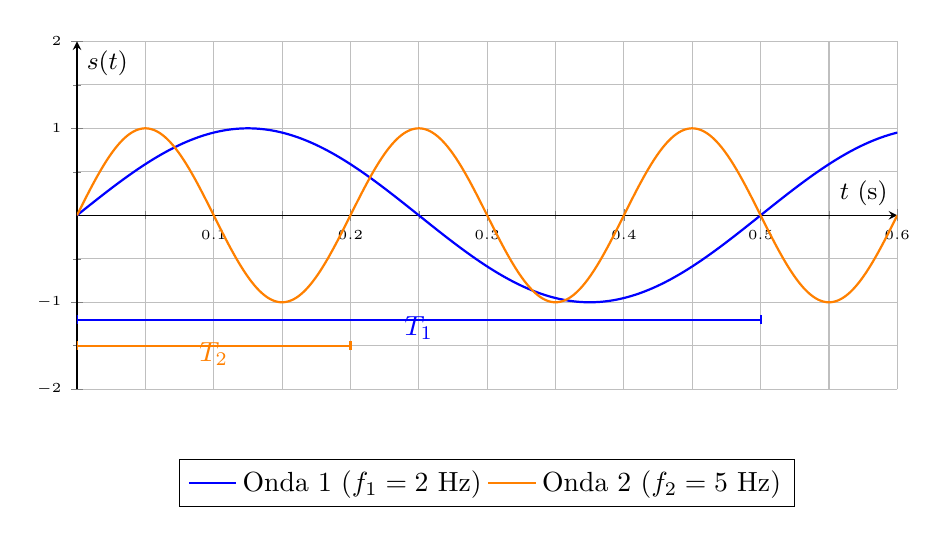
\begin{tikzpicture}
\begin{axis}[
    width=12cm, height=6cm,
    axis lines = middle,
    xlabel = {$t$ (s)},
    ylabel = {$s(t)$},
    label style={font=\small},
    tick label style={font=\tiny},
    grid = both,
    minor tick num = 1,
    domain = 0:0.6,
    samples = 500,
    xmin=0, xmax=0.6,
    ymin=-2, ymax=2,
    legend style={at={(0.5,-0.2)}, anchor=north, legend columns=-1}
]

% Onda 1: 2 Hz
\addplot [blue, thick] {1 * sin(deg(2 * pi * 2 * x))};
\addlegendentry{Onda 1 ($f_1=2$ Hz)}

% Onda 2: 5 Hz
\addplot [orange, thick] {1 * sin(deg(2 * pi * 5 * x))};
\addlegendentry{Onda 2 ($f_2=5$ Hz)}

% Barra indicando período Onda 1
\addplot [blue, thick] coordinates {(0,-1.2) (0.5,-1.2)};
\addplot [blue, thick] coordinates {(0,-1.25) (0,-1.15)};
\addplot [blue, thick] coordinates {(0.5,-1.25) (0.5,-1.15)};
\node[blue] at (axis cs:0.25,-1.3) {$T_1$};

% Barra indicando período Onda 2
\addplot [orange, thick] coordinates {(0,-1.5) (0.2,-1.5)};
\addplot [orange, thick] coordinates {(0,-1.55) (0,-1.45)};
\addplot [orange, thick] coordinates {(0.2,-1.55) (0.2,-1.45)};
\node[orange] at (axis cs:0.1,-1.6) {$T_2$};

\end{axis}
\end{tikzpicture}
\end{center}